%-------------------------------------------------------------------------------
% yum_menu_instruments
%-------------------------------------------------------------------------------
%
% \file        yum_menu_instruments.tex
% \library     Documents
% \author      Chris Ahlstrom
% \date        2016-02-27
% \update      2016-10-15
% \version     $Revision$
% \license     $XPC_GPL_LICENSE$
%
%     Provides the Menu / Instruments section of yoshimi-user-manual.tex, for
%     the 1.3.8 and above versions of Yoshimi.  That menu entry has changed a
%     lot.
%
%-------------------------------------------------------------------------------

\subsection{Menu / Instruments}
\label{subsec:menu_instrument}

   The \textsl{Yoshimi} Instruments menu lets one select instruments and work
   with banks of instruments.
   \textsl{Yoshimi} stamps instrument XML files with its own major and minor
   version numbers so it is possible to tell which version created the files,
   or whether they were created by \textsl{ZynAddSubFX}.

   While the \textbf{Instrument Menu} allows for the management of parts, the
   \textbf{Part Edit} dialog, described in
   \sectionref{subsec:bottom_panel_instrument_edit},
   is where one would start for the the creation of a new part/instrument.

   When opening an instrument bank one can now tell exactly which synth engines
   are used by each instrument. This is represented by three pale background
   colours:

   \begin{itemize}
      \item \textbf{\textcolor{red}{Red}}: ADDsynth
      \item \textbf{\textcolor{blue}{Blue}}: SUBsynth
      \item \textbf{\textcolor{green}{Green}}: PADsynth
   \end{itemize}

   These new colored engine backgrounds aren't just pretty. They give real
   information about expected processor load, and time taken to be ready when
   loaded:

   \begin{itemize}
      \item Processor Load, low to high:
         \textbf{\textcolor{green}{PAD}},
         \textbf{\textcolor{blue}{SUB}}, then
         \textbf{\textcolor{red}{ADD}}.
      \item Time to initialize, low to high:
         \textbf{\textcolor{blue}{SUB}},
         \textbf{\textcolor{red}{ADD}},
         \textbf{\textcolor{green}{PAD}}.
   \end{itemize}

   If the instruments are kits they scanned to find out if 
   \textsl{any} member of the kit contains each engine.
   This scanning is duplicated in the current part, the mixer panel for the
   currently loaded instruments, and in the Instrument Edit window the same
   colors highlight the engine names when they are enabled with the check
   boxes. 

   The following sub-menus are provided, as shown in
   \figureref{fig:yoshimi_instrument_menu}.

\begin{figure}[H]
   \centering 
   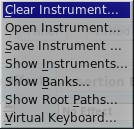
\includegraphics[scale=0.9]{1.3.8/yoshimi-menu-instrument.jpg}
   \caption{Yoshimi Menu, Instrument}
   \label{fig:yoshimi_instrument_menu}
\end{figure}

   This new version of the \textbf{Instrument} menu is somewhat different than
   the old version.  It is actually simpler and easier to use, while still
   offering all of the power of the setting up of instruments in
   \textsl{Yoshimi}.

   \begin{enumber}
      \item \textbf{Show Stored...}
      \item \textbf{Load External...}
      \item \textbf{Save External...}
      \item \textbf{Clear}
   \end{enumber}

%  \setcounter{ItemCounter}{0}      % Reset the ItemCounter for this list.

\subsubsection{Menu / Instrument / Show Stored...}
\label{subsubsec:menu_instrument_show}

   Instruments are stored in banks
   (see \sectionref{subsec:concepts_banks_and_roots}).
   The banks (and current bank setting) are
   loaded/saved automatically by the program, so one doesn't have to worry
   about saving the banks before the program exits. On program start, the last
   used bank is loaded. A single bank can store up to 128 instruments.
   However, there is space for a number of additional instruments in the bank,
   the extended-program section, to allow up to 160 instruments in a bank.

   When the \textbf{Show Stored...} button is selected, a dialog comes
   up that shows all of the instruments present in the currently-selected
   bank.
   
\begin{figure}[H]
   \centering 
%  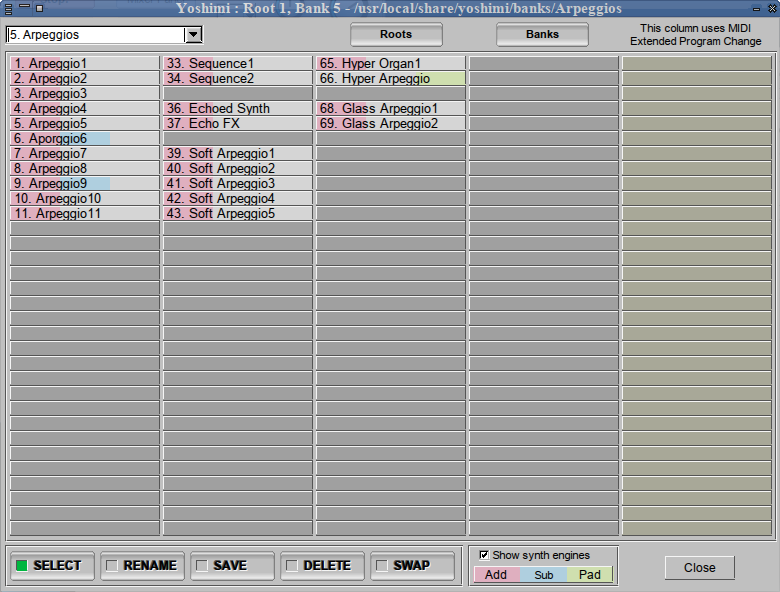
\includegraphics[scale=0.75]{1.3.9/instruments_show_stored.png}
   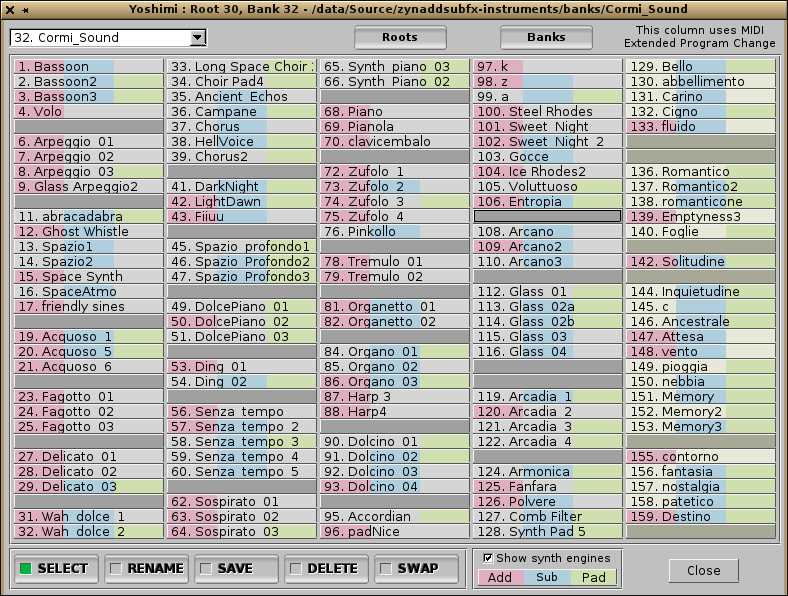
\includegraphics[scale=0.75]{1.4.1/Instrument.png}
   \caption[Show Stored Instruments]{Instruments Stored in Current Banks}
   \label{fig:instruments_show_stored}
\end{figure}

   As \figureref{fig:instruments_show_stored},
   shows, this is a very complex dialog with a lot of options.
   The figure shows a default setup, with the first bank of instruments,
   \textbf{5. Arpeggios}, listed.
   If one drops this list down (shown later), one also observes that the banks
   are numbered in increments of 5, to make it easier for a user to insert his
   or her own bank(s) of instruments.

   The default set of banks are spaced 5 apart only because thats the
   best-fit for the current number of banks.  If we add more banks in future
   versions of \textsl{Yoshimi}, then a \textsl{clean} install is likely to have
   different spacing, but for an existing setup, the new entries will just be
   slotted in where they will fit.

   Also, if one deletes banks or instruments by some external means, the next
   time \textsl{Yoshimi} starts, it will notice their absence and quietly
   remove their entries.

   Note how \textsl{Yoshimi} now shows the color codings for the
   synth-sections used in each instrument:
   red for ADDsynth, blue for SUBsynth, and green for PADsynth.

   Also note how the numbers at the beginning of the filenames are used as
   an "instrument" or "program" number.  These numbers can be used in MIDI
   Program Change commands.
   
   All of the instrument files (such as \texttt{0001-Arpeggio1.xiz})
   with filenames starting with numbers (no matter how many digits)
   will be
   shown in the corresponding slot number.  Those instrument files
   without numbers (or larger numbers?) will start
   with numbers at 129 or above ("Extended Program Change") up to 160.
   One could give them numbers by renaming them outside of \textsl{Yoshimi},
   then reloading the bank.
   One can also fix unnumbered ones simply by loading them, then resaving them
   to the same slot. It's then probably best to swap them into the main set,
   if there is space.

   \index{extended program}
   Note that MIDI CC
   (see \sectionref{paragraph:menu_yoshimi_settings_ccs})
   can be set to access voices from 129 to 160.
   All the Bank controls in the \textbf{MIDI} settings tab take immediate
   effect when set.
   Bank and program changes can be completely disabled in the settings tab;
   some hardware synths don't play nice with it.

   Learning how to use the Instruments dialog is an important way to make
   instruments easier to manage, and so this will be a long discussion.

%  An important pair of concepts in \textsl{Yoshimi} are
%  \textsl{banks} and \textsl{roots}.  These concepts are described in
%  \sectionref{subsec:concepts_banks_and_roots}.

   Here is a list of the user-interface items in the instruments/banks dialog:

   \begin{enumber}
      \item \textbf{Bank Names}
      \item \textbf{Roots}
      \item \textbf{Banks}
      \item \textbf{Instrument and Bank Matrix}
      \item \textbf{SELECT}
      \item \textbf{RENAME}
      \item \textbf{SAVE}
      \item \textbf{DELETE}
      \item \textbf{SWAP}
      \item \textbf{Show synth engines}
         (was \textbf{Show PADsynth status})
      \item \textbf{Close}
   \end{enumber}

   \setcounter{ItemCounter}{0}      % Reset the ItemCounter for this list.

   \itempar{Bank Names}{instruments!bank names}
   Instruments Bank Name.
   This item is a drop-down list of the available instrument banks in the
   currently-selected \textbf{root} directory.
   Basically, each bank is a directory name, with a number prepended.
   The banks are found under the current root, which is a also a directory
   name, and is the name of the parent directory of a set of banks.
   Here is the Bank Names drop-down list for the default setup, which has the
   default banks provided by the basic \textsl{Yoshimi} installation.

\begin{figure}[H]
   \centering 
%  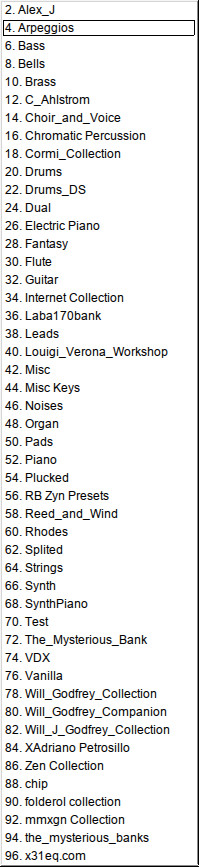
\includegraphics[scale=0.75]{menu/Instrument/bank-list.jpg}
   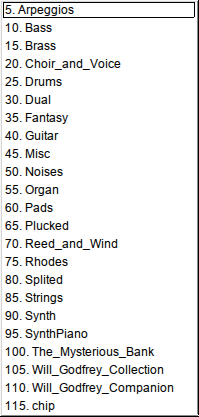
\includegraphics[scale=0.75]{1.3.9/instruments_bank_list.png}
   \caption[A Sample Bank List]{A Sample Bank List}
   \label{fig:bank_list}
\end{figure}

   And here is the directory listing associated with it, in the order
   produced by the UNIX/Linux \texttt{ls -1}
   (list single-column) command (shown in
   two columns to save space):

   \begin{verbatim}
      Arpeggios          Pads
      Bass               Plucked
      Brass              Reed_and_Wind
      chip               Rhodes
      Choir_and_Voice    Splited
      Drums              Strings
      Dual               Synth
      Fantasy            SynthPiano
      Guitar             The_Mysterious_Bank
      Misc               Will_Godfrey_Collection
      Noises             Will_Godfrey_Companion
      Organ              
   \end{verbatim}

   The directories (banks) shown above come from the default \textbf{root}
   when \textsl{Yoshimi} and its data files are installed:
   \texttt{/usr/share/yoshimi/banks}.
   If one installed \textsl{Yoshimi} by building the source code, then
   this directory will be
   \texttt{/usr/local/share/yoshimi/banks}.

   The first thing to note is that there are only 128 \textsl{Yoshimi} banks
   supported in a \textsl{Yoshimi} root.
   If the list of banks takes up about
   half of the available slots, it might be time to move some of those banks to
   a new root directory.

   The numbers in the drop-down list are generated by \textsl{Yoshimi} the
   first time it sees a new root path or a new bank within the root path.
   Once set, these numbers will never change unless one actually moves them
   around (using the \textbf{SWAP} button).

   The bank number is also the MIDI ID for the bank;
   one can be sure that it will always
   be there for bank changes, no matter how many banks are added later.
   \textsl{Yoshimi} always lists the banks in ID order, not alphabetical
   order, so one can group them sensibly and permanently.
   However, at first-time creation \textsl{Yoshimi} sets the IDs in
   alphabetical order and tries to space them evenly over the range to
   provide some wiggle room.                                        

   Selecting one of the items in this drop-down list selects the bank and
   loads it into the Banks dialog.

   \index{anti-auto-clutter}
   Right- or left-clicking on a bank in the drop-down list
   causes the instrument list of the previous bank to be replaced by the
   instrument list of the newly-selected bank.

   \itempar{Roots}{instruments!roots}
   Instruments Roots Button.
   Shows a list of directories that can serve as "root" directories.
   The "Bank Root Paths" dialog discussed in
   \sectionref{subsubsec:menu_patch_sets_patch_bank_roots} in
   \figureref{fig:show_patch_banks}, shows
   the system root (e.g. \texttt{/usr/share/yoshimi/banks}) and
   a user's home location for his/her banks and roots.

   \itempar{Banks}{instruments!banks}
   Banks Button.
   This item brings up a Banks dialog showing all of the banks present in the
   current root.
   It is an alternative to using the \textbf{Bank Names} drop-down list to
   select a bank.  It is also a way to reorganize and renumber the
   banks without using the Linux console or a file-explorer application to do
   so.

   \itempar{Instrument and Bank Matrix}{instruments!bank matrix}
   Instruments Bank Matrix.
   Shows the instruments that are in the currently selected bank
   (directory).

   The next few items are selector buttons that determine what happens when one
   clicks on an instrument name.

   \itempar{SELECT}{instruments!SELECT}
   Instruments SELECT.
   When this button is selected, then clicking on an instrument selects that
   instrument as the instrument for the current Part active in the main
   window.  In the main window of \textsl{Yoshimi}, that instrument name will
   appear in the currently-selected \textbf{Part}.  If \textsl{Yoshimi} is
   writing to a console window then each part, when clicked, will be shown:

   \begin{verbatim}
		yoshimi> Loaded 64 "Hyper Organ1" to Part 0
		Loaded 65 "Hyper Arpeggio" to Part 0
		Loaded 10 "Arpeggio11" to Part 0
		Loaded 41 "Soft Arpeggio4" to Part 0
		Loaded 67 "Glass Arpeggio1" to Part 0
   \end{verbatim}

   (Remember that "Part 0" in the console is actually "Part 1" in the main
   window.)

   \itempar{RENAME}{instruments!RENAME}
   Instruments RENAME.
   When this button is selected, then clicking on a bank brings
   up a small dialog to rename the clicked-on bank.
   However, one will see the following warning message if trying to rename a
   file that is in a directory not modifiable by normal users:

   \begin{verbatim}
      ! Could not rename instrument 39 to Soft Arpeggio5 [Close]
   \end{verbatim}

   Note that, as soon as this operation is done, the auto-selector (green
   check-box) moves back to the \textbf{SELECT} button.

   \itempar{SAVE}{instruments!SAVE}
   Instruments SAVE.
   When this button is selected, then clicking on a bank saves
   the instruments as currently configured.
   A prompt like the following will appear:

   \begin{verbatim}
      ? Overwrite the slot no. 43 ?  [No/Yes]
   \end{verbatim}

   However, if one answers yes, and the instrument is in a non-modifiable
   directory, then one will see the following error message:

   \begin{verbatim}
      ! Could not save to this location [Close]
   \end{verbatim}

   \itempar{DELETE}{instruments!DELETE}
   Instruments DELETE.
   Selecting this button and clicking an empty bank entry does nothing.
   Selecting this button and clicking an existing bank entry brings up a
   small dialog asking one if this bank is really to be deleted.

   \begin{verbatim}
      ? Clear the slot no. 68?  [No/Yes]
   \end{verbatim}

   However, if one answers yes, and the instrument is in a non-modifiable
   directory, then one will see the following error message:

   \begin{verbatim}
      ! Could not clear this location  [Close]
   \end{verbatim}

   \itempar{SWAP}{instruments!SWAP}
   Instruments SWAP.
   Selecting this button, then selecting one instrument, and then another,
   swaps the numbering and postion of the selected instruments.
   However, one might also experience the following warning message:

   \begin{verbatim}
      ! Could not swap these locations  [Close]
   \end{verbatim}

   Note that all of the above error messages are also shown in the console, if
   it is where \textsl{Yoshimi} is running.  For example:

   \begin{verbatim}
      40 Failed to remove /usr/local/share/yoshimi/banks/Arpeggios/0041-Soft
      Arpeggio3.xiz Permission denied
   \end{verbatim}

   \itempar{Show synth engines}{instruments!show engines}
   If enabled, then the usage of each of the \textsl{Yoshimi} synthesis
   engines is indicated by color coding, as shown in the figure above.

   \itempar{Close}{instruments!Close}
   Closes the window.

%  Here is a more conventional view of instruments, supplied with
%  \textsl{Yoshimi}, shown in
%  \figureref{fig:show_pads_bank}.
% 
% \begin{figure}[H]
%    \centering 
% %  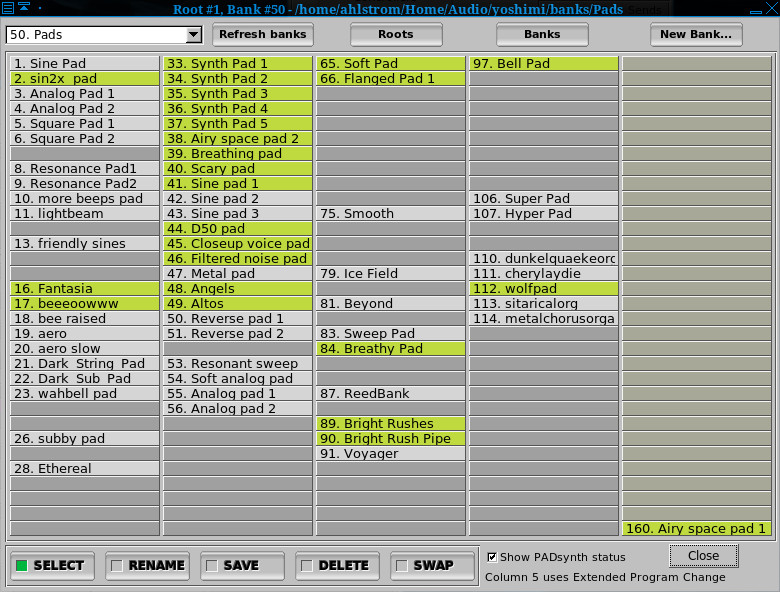
\includegraphics[scale=0.75]{menu/Instrument/show-pads-bank.jpg}
%    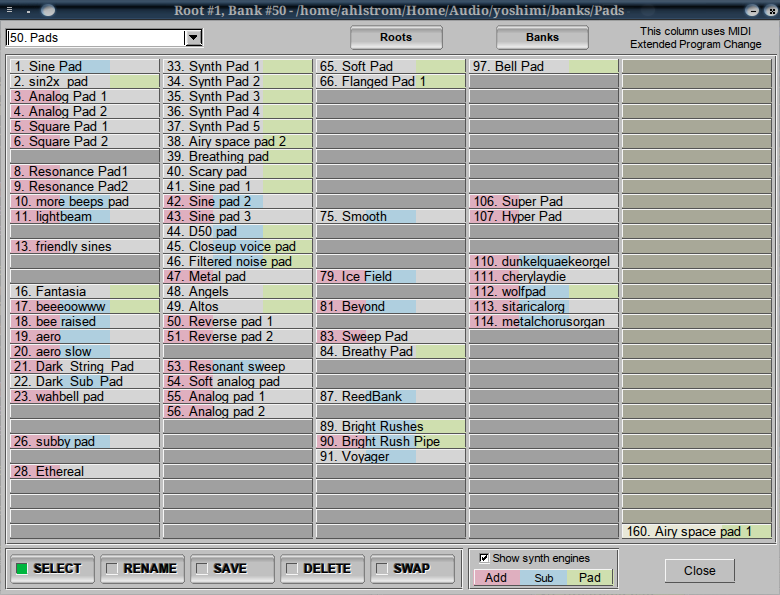
\includegraphics[scale=0.75]{1.3.6/show_pads_bank.png}
%    \caption[Show Pads Instruments]{Show Pads Instruments}
%    \label{fig:show_pads_bank}
% \end{figure}
% 
%    Note that many of these Pads instruments also use the Add and Sub
%    components as well.

\subsubsection{Menu / Instrument / Load External...}
\label{subsubsec:menu_instrument_load}

   This menu entry simply brings up a file dialog, allowing the user to
   navigate to an arbitrary directory, and then to a solitary instrument file
   (\texttt{*.xiz}), and load it into the current Part.

\begin{figure}[H]
   \centering 
   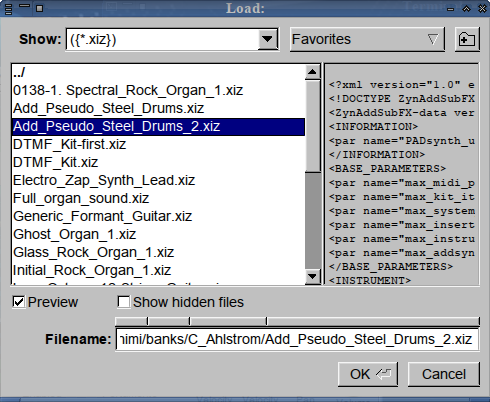
\includegraphics[scale=0.75]{1.3.9/instruments_load_external.png}
   \caption{Instruments, Load External}
   \label{fig:instruments_load_external}
\end{figure}

   These "xiz" files are normally found in a \texttt{banks} directory, but this
   operation allows access to instruments that are not located in a bank.

   This dialog has a number of user-interface elements to discuss:

   \begin{enumber}
      \item \textbf{Show}
      \item \textbf{Favorites}
      \item \textbf{Create a new diretory}
      \item \textbf{Instrument List}
      \item \textbf{XML Preview}
      \item \textbf{Preview}
      \item \textbf{Show hidden files}
      \item \textbf{Directory Bar}
      \item \textbf{Filename}
      \item \textbf{OK}
      \item \textbf{Cancel}
   \end{enumber}

   These elements are used in a number of different places in \textsl{Yoshimi}.
   Therefore, we will explain them all once, here.

   \setcounter{ItemCounter}{0}      % Reset the ItemCounter for this list.

   \itempar{Show}{Load External!show}
   Show types of files.
   This item shows a file filter for selecting instrument files.
   The types of filters are as follows (screen shot not available):

   \begin{enumber}
      \item \textbf{(\{*.xiz\})} (compressed XML files)
      \item \textbf{All Files (*)}
      \item \textbf{Custom Filter}
   \end{enumber}

   \itempar{Favorites}{Load External!favorites}
   Favorite directories.
   Provides a list of options and favorite directories in which to find 
   instrument files.

\begin{figure}[H]
   \centering 
   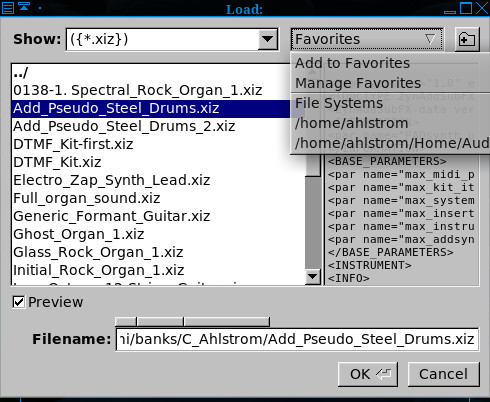
\includegraphics[scale=0.75]{menu/Instrument/favorites-dropdown.jpg}
   \caption{Manage Favorites Drop-Down List}
   \label{fig:open_instrument_favorites}
\end{figure}

   \begin{enumber}
      \item \textbf{Add to Favorites}
      \item \textbf{Manage Favorites}
      \item \textbf{File Systems}
      \item \textbf{\textsl{(current favorite directories)}}
   \end{enumber}

   \index{Add to Favorites}
   \textbf{Add to Favorites}
   simply adds the currently selected directory shown in the instrument list
   to the list of favorites.

   To add favorites in the file dialog, navigate to the desired directory.
   Then click \textbf{Favorites}, and select \textbf{Add to Favorites}.

   Once one has a number of favorites set up,
   there is a \textbf{Manage Favorites} that can be used.
   For example, if one needs to get rid of a directory, one can use the
   \textbf{Manage Favorites}
   \index{Manage Favorites}
   dialog, shown in
   \figureref{fig:manage_instrument_favorites} below,
   to do that.

\begin{figure}[H]
   \centering 
   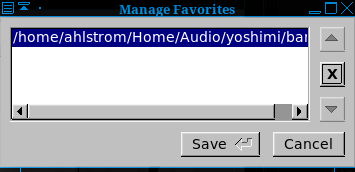
\includegraphics[scale=0.75]{menu/Instrument/manage-favorites.png}
   \caption{Manage Favorites Dialog}
   \label{fig:manage_instrument_favorites}
\end{figure}

   \textbf{File Systems} \index{File Systems}
   Provides a list of all file systems starting at root ("\texttt{/}").
   This list can be pretty confusing, with a lot of entries.
   But note that one navigates to ("\texttt{/}"), and from there to
   \texttt{/usr/share/yoshimi/banks} to get easy access to all the
   instruments that are preinstalled with
   \textsl{Yoshimi}.
   Generally, one will want to use only
   \textbf{Add to Favorites} and \textbf{Manage Favorites}.

   \itempar{Create Directory}{Load External!create new directory}
   Creates a New Directory.
   This little symbol brings up a small "New Directory?" dialog (not shown
   here, it is very simple and stock) into which one can type a directory
   name to be added to the current directory of the instrument list.

   \itempar{Instrument List}{Load External!instrument list}
   Provides a list of the instrument files available in the current
   directory.  Also shown are sub-directories (if available)
   that might contain more instruments, and a ("\texttt{../}") entry
   to navigate to the parent directory.

   \itempar{Preview}{Load External!preview checkbox}
   If one thinks the preview feature is not useful, uncheck this check-box.
   so that one doesn't see the preview window.  As a bonus, one can see more
   of a long instrument file-name.

   \itempar{Preview pane}{Load External!preview pane}
   XML Preview.
   This box can show the beginning of the XML data of an instrument file.
   \textbf{Bug:}
   \index{bugs!compressed XML preview}
   The XML preview feature shows the XML only if the XML is not compressed.

   \itempar{Show hidden files}{Load External!show hidden files}
   Shows file that are hidden.  Not sure how useful this feature is;
   who would hide a \textsl{Yoshimi} instrument file?

   \itempar{Directory Bar}{Load External!directory bar}
   Provides an alternate way to move up through the directory structure.
   Click on each of the small bevelled rectangles to move around in the
   directory hierarchy.

   \itempar{Filename}{Load External!filename}
   File Name.
   Provides the full path specification for the instrument file.

   \itempar{OK/Cancel}{Load External!ok/cancel}
   We don't really need to discuss the \textbf{OK} and \textbf{Cancel}
   buttons, do we?  OK, we'll cancel that discussion.

\subsubsection{Menu / Instrument / Save External...}
\label{subsubsec:menu_instrument_save}

   This menu entry simply brings up a file dialog, allowing the user to
   navigate to an arbitrary directory, and then save the current Part
   to a solitary instrument file (\texttt{*.xiz}).

\begin{figure}[H]
   \centering 
   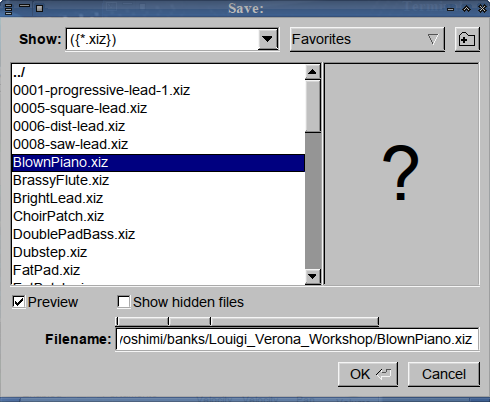
\includegraphics[scale=0.75]{1.3.9/instruments_save_external.png}
   \caption{Instruments, Save External}
   \label{fig:instruments_save_external}
\end{figure}

   This dialog is very similar to the \textbf{Load External} dialog.
   Note the large question mark in the XML preview, indicating a compressed XML
   file.  If uncompressed, then an XML text preview will be shown.

   The instrument save action saves only what is essential to the instrument,
   and not the part it may be sitting in.  If there have been no changes in the
   instrument, then a \textbf{Nothing to save!} dialog appears.

\subsubsection{Menu / Instrument / Clear}
\label{subsubsec:menu_instrument_clear}

   This menu entry simply clears the instrument that is loaded into the current
   Part.  This converts the instrument to a 
   \textsl{Simple Sound} patch.
   This menu entry brings up a prompt to clear the parameters of the
   instrument that is currently loaded in the current part.

\begin{figure}[H]
   \centering 
   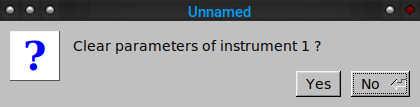
\includegraphics[scale=0.75]{menu/Instrument/clear-instrument.jpg}
   \caption{Clear Instrument Dialog}
   \label{fig:clear_instrument_dialog}
\end{figure}

   Funny, in recent versions of \textsl{Yoshimi}, the \textbf{Yes} and
   \textbf{No} buttons have switched places.  \textbf{No} is now the default
   action.

%-------------------------------------------------------------------------------
% vim: ts=3 sw=3 et ft=tex
%-------------------------------------------------------------------------------
